\documentclass[a4paper]{sbgames}               % final
%\usepackage[scaled=.92]{helvet}
\usepackage[latin1]{inputenc}   % pacote para acentua��o
\usepackage{times}
\usepackage{graphicx}

%% use this for zero \parindent and non-zero \parskip, intelligently.
\usepackage{parskip}

%% the 'caption' package provides a nicer-looking replacement
\usepackage[labelfont=bf,textfont=it]{caption}

\usepackage{url}

%% Paper title.
\title{Charack: tool for real-time generation of pseudo-infinite virtual worlds for 3D games}

%% Author and Affiliation (multiple authors). Use: and between authors

\author{%Fernando Bevilacqua\\ Cesar Tadeu Pozzer \\ Universidade Federal de Santa Maria 
        %\and Name2 B. Surname2\\ Name3 C. Surname3\\ ZZZZ University
        Paper 60326\\ 
}
\contactinfo{%\{fernando,pozzer\}@inf.ufsm.br
}
%% Keywords that describe your work.
\keywords{MMO, virtual worlds, terrain generation, 3D games, noise, procedural generation, multifractal}

%% Start of the paper
% Attention: As you need to insert EPS images in Postscript, 
% you need to insert PDF images into PDFs. 
% In the text, extensions cancbe omitted (latex use .eps, pdflatex get .pdf) 
% To convert them: epstopdf myimage.eps
\begin{document}

\teaser{
  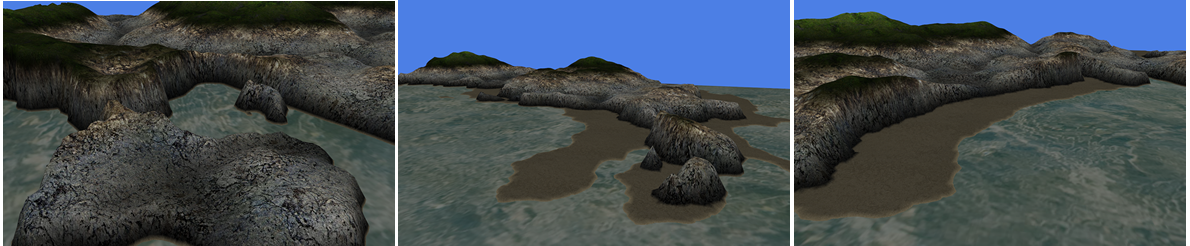
\includegraphics[width=\linewidth]{images/teaser.png}
  \caption{Coastlines and islands procedurally generated by Charack}
}

%% The ``\maketitle'' command must be the first command after the
%% ``\begin{document}'' command. It prepares and prints the title block.

\maketitle

%% Abstract section.

\begin{abstract}
In MMO games the player's experience is mainly influenced by the size and details of the virtual world. Technically the bigger the world is, the bigger is the time the player takes to explore all the places. This work presents a tool (named Charack) able to generate pseudo-infinite virtual worlds with different types of terrains. Using a combination of algorithms and content management methods, Charack is able to create beaches, islands, bays and coastlines that imitates real world landscapes. The tool clearly distinguish the generation of each type of content. The contribution of the tool is the ability to generate giant pieces of land (or landscape) focusing on detailed coastline generation, by means of using procedural algorithms.
\end{abstract}

%% The ``\keywordlist'' command prints out the keywords.
\keywordlist
\contactlist

%%%%%%%%%%%%%%%%%%%%%%%%%%%%%%%%%%%%%%%%%%%%%%%%%%%%%%%%%%%%%%%%%%%
\section{Introduction}
%%%%%%%%%%%%%%%%%%%%%%%%%%%%%%%%%%%%%%%%%%%%%%%%%%%%%%%%%%%%%%%%%%%

The computer games market has been evolving considerably over the years. Since the first console, the hardware performance has increased and new graphic technologies were developed, resulting in a wide range of themes and game styles. In the multiplayer games, players interact with other human beings and also with NPCs, which are represented by virtual characters. That kind of game is popular and the social interaction between players is a matter of research ~\cite{onlineGaming,ducheneaut}. In the category of multiplayer games there are the massively multiplayer on-line (MMO) ones, which are on-line games featuring large number of players interacting with each other in a huge virtual world.

An MMO can feature millions of players, such as EverQuest ~\cite{EverQuest} and World of Warcraft ~\cite{Blizzard}, the latter with more than 6 million subscribers ~ \cite{vicioEstrutura}. A persistent virtual world is an important topic to keep the game fun and attractive to the player. The bigger is the world to be explored, technically the bigger is the time the player has to spend in order to explore all the places. As a result of such huge virtual worlds, their creation and subsequent upgrade are a complex task. EverQuest and World of Warcraft present a virtual world with a wide diversity of geographical features such as mountains, valleys, forests, fields, caves, etc, and most of them have specific names  and are related to the game story. The manual creation of those virtual worlds requires a team able to design heightmaps, adorn landscapes, ensure usability of the map (avoid unreachable places, for instance), create interesting places for players, etc. To help on that task, the development of a tool able to generate complex virtual worlds is useful to speed up the development of 3D games such as MMOs.

The solution proposed in this work is the development of a tool, called Charack, able to generate complex virtual worlds in real-time using noise-based techniques for terrain generation. Charack was designed to allow developers to use its features in order to generate 3D terrains for games, particularly MMOs, with minimal human intervention in the generation process. The content generation is made on demand. As the user moves along the world, the elements inside the user's view are processed and stored into the memory and the ones away from the user's view are removed. Even though the generation of all elements is based on random numbers, if the player visits an specific point {\tt A}, then walks for miles generating a completely different set of landscapes, and returns to point {\tt A}, the same previously seen landscape will be shown again.

Charack handles separately the content generation of continents, topography and coastlines, so each of those elements can be independently adjusted in order to produce highly customized results. The use of the term "pseudo" is necessary due physical limitations in computers hardware: an unsigned integer, for instance, can store a certain amount of data; if there were no physical limitations, the tool would be able to generate, in fact, an infinite world.

This paper is organized as follows. Section ~\ref{sec:related-work} describes related work concerning the generation of finite or infinite virtual worlds. Section ~\ref{sec:tool-organization} presents the tool structure and the techniques used in the content generation process. Section ~\ref{sec:results} describes and illustrates the results that Charack produced. Finally section ~\ref{sec:conclusion} presents a conclusion and ideas for future work.

%%%%%%%%%%%%%%%%%%%%%%%%%%%%%%%%%%%%%%%%%%%%%%%%%%%%%%%%%%%%%%%%%%%
\section{Related works}
\label{sec:related-work}
%%%%%%%%%%%%%%%%%%%%%%%%%%%%%%%%%%%%%%%%%%%%%%%%%%%%%%%%%%%%%%%%%%%

There are several related works concerning the generation of finite or infinite virtual worlds. One of them creates an infinite city that is presented to the user on demand as it walks on the ground~\cite{infinicity}. The world were divided into a grid composed of several squares, called cells. The location of each cell is used with a global seed as an input for a hash function ~\cite{wangHash}. The result of this function is used as a seed for a pseudo random number generator and it defines all the characteristics of the buildings within a cell. As a consequence of that approach the contents of a cell is always the same, no matter if the user moves and that cell is removed from the memory. That work was the ground zero for Charack development, however the original idea was changed in order to make the tool suitable to generate more types of terrains (mountains, plains, continents, etc.), not only streets and buildings. The approach of content generation made on demand was maintained, but the cells organization was removed.

The use of a procedurally generated world approach ~\cite{LindaOndrej2007} is very close to the concept of content generation aimed for Charack. In that work, a spherical planet is created as a result of a recursive division of a geometric shape, then noise functions are applied to the mesh to generate the heightmap. There is no distinction between the content generation approach for continents and the content generation for the terrain within the continents. As a result the continents are created by flooding the heightmap with a water plane, which will produce the coastlines based on the sea level height and the amount of ripples in the topography. The content itself is not generated on demand. Charack was created from an evolution of that idea, but with limitations. The world created by Charack handles differently the content generation of continents, coastlines and the heightmap and it also generates the content on demand, however it does not use a spherical approach.

Another related work was a tool used to build the SkyCastle multiplayer game engine~\cite{LandscapeGeneration,SkyCastle}. For the heightmap generation, parameterized procedures and fractal based systems are combined in a layered approach: starting with a base map, the application merges a new map with the base one in each iteration. The new maps are pre-calculated and generated using Perlin noise~\cite{Perlin85}. To texturize the landscape and to adorn it with plants, several techniques are used ~\cite{CSHD03,PL90,LD98,WP95}. Charack uses a similar noise approach in order to create the terrain height, however it was not initially designed to generate extra content such as trees and plants.

The generation of a virtual world as a result of recursive subdivisions of a quadtree ~\cite{dollins-thesis} is very similar to the Charack proposal. In that work, a world with huge proportions is created and its content is generated on demand as the user moves. The heightmap is created in a parameterized and multi-resolution way, so the closer the user is of place, the greater is the amount of detail there. There is also no distinction in the content generation process of continents, coastlines and land. The proposed heightmap generation is used by Charack, however continents and the coastlines generation process are completely different.

Another approach uses fractals affected by erosion for real-time, procedural generation of terrains ~\cite{terrain_generation}. For the erosion simulation, thermal ~\cite{MusgraveErosao} and hydraulic methods are used. Charack has no feature connected with the weather influence, even though it produces some sort of very basic erosion simulation when all sharp edges of the heightmap are removed by a smoothing algorithm.

The planet map creator based on the generation of a spheric world using a recursive subdivision of a tetrahedron is another approach concerning procedural content generation~\cite{torben}. All the generated information is part of a complete virtual world featuring highly customizable continents and oceans created as a result of a projection of pixels onto a sphere, a method similar to ray tracing~\cite{raytracing}. That planet map creator is used by Charack as a starting point on the continent generation process. Figure ~\ref{fig:explicacao_torben_resultado} illustrates the planet map creator results.

\begin{figure}
\centering
\resizebox{8cm}{!}{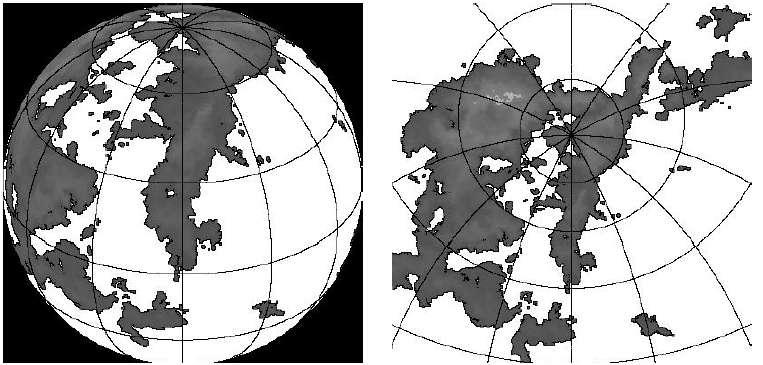
\includegraphics{images/explicacao_torben_resultado.png}}
\caption{Results of the planet map creator used by Charack}
\label{fig:explicacao_torben_resultado}
\end{figure}

%%%%%%%%%%%%%%%%%%%%%%%%%%%%%%%%%%%%%%%%%%%%%%%%%%%%%%%%%%%%%%%%%%%
\section{Tool organization}
%%%%%%%%%%%%%%%%%%%%%%%%%%%%%%%%%%%%%%%%%%%%%%%%%%%%%%%%%%%%%%%%%%%
\label{sec:tool-organization}

%%%%%%%%%%%%%%%%%%%%%%%%%%%%%%%%%%%%%%%%%%%%%%%%%%%%%%%%%%%%%%%%%%%%%
\subsection{Basic structure}
\label{sec:basic-structure}
%%%%%%%%%%%%%%%%%%%%%%%%%%%%%%%%%%%%%%%%%%%%%%%%%%%%%%%%%%%%%%%%%%%%%

Analyzing the related works, virtual worlds are generated through several approaches, but none of them handles differently the content generation for continents, coastlines and topography. Although there are variations in how the heightmap is created, the generation of continents is a result of a water flooding plane. This method allows the developers to focus on the content generation for the land, however it has a simple approach concerning continents and coastlines. The main idea and contribution of Charack is the content generation handled differently for each world element (continent, coastline, etc.), with an aggressive and specific approach for each one. This is a new approach for the content generation process, which is different from the the related works that focuses on content generation as a unified process.

In order to create a virtual world that reaches the presented proposal, a top-down plan is used for the content generation. The Charack data flow begins in a macro view of the world, which are the continents, evolving to a micro view of the planet, which are the content generation for each vertex that will be drawn in the screen. Figure ~\ref{fig:planejamento_estrutura_basica} shows Charack basic structure.

\begin{figure}
\centering
\resizebox{7cm}{!}{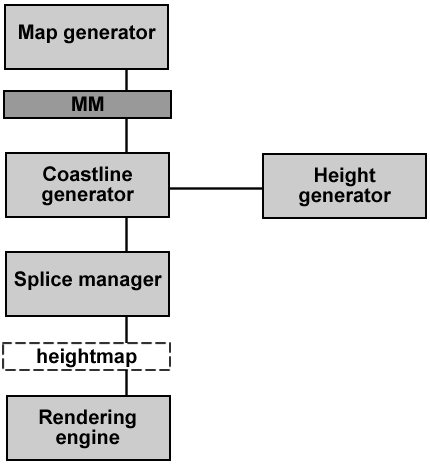
\includegraphics{images/english/planejamento_estrutura_basica.png}}
\caption{Charack's basic structure}
\label{fig:planejamento_estrutura_basica}
\end{figure}

\subsubsection{Maps generator}

At the top of the chain is the map generator, which creates the continents that exist throughout the virtual world. This module is an encapsulation of the solution created by ~\cite{torben}. When the tool is initiated, it uses a user defined seed to generate all the continents. Once the continents are generated, all the information related to terrain types (land, water and coast) are stored in a matrix called {\bf macro-matrix (MM)}, which is used by all the other algorithms.

\subsubsection{Slice manager}

Below the MM and the map generator is the slice manager (SM). It extracts a portion of the virtual world (the user's view) and provide the rendering engine with information about the heightmap. In order to obtain the required information to create the heightmap, the slice manager uses the coastline generator (CG), which uses the height generator (HG) and the data stored in the MM.

In the context of the SM, there is no information about land or water, only a set of vertexes and their height values. Using the position of the user as a guide, the SM slices the virtual world and, for each collected vertex, it queries the CG in order to find out the height value for that vertex.

\subsubsection{Height generator}

The height generator (HG) defines the height value for each vertex in the virtual world. To ensure that the developers can create a customizable heightmap based on their needs, new functions to generate content can be added to the tool in a simple way.

\subsubsection{Coastline generator}

The coastline generator (CG) will map each vertex of the slice manager to the MM in order to find out the terrain type of that vertex. If the vertex being analyzed is mapped to a location in the MM that is described as water, then the CG assigns a height value equals to sea level for that vertex and returns it to the SM. If the vertex is mapped to a place described as (simple) land, then the CG will use the information provided by the HG in order to set the height value for that vertex. Finally, if the vertex is mapped to a place described as coast, then the CG uses its own structure (together with the MM) to set the height value for the that vertex.

The resulting virtual world technically has height and width defined by the maximum size of a signed integer, however it is physically impossible to generate a MM with such proportions. Since the MM is smaller than the virtual world, an MM's entry {\tt (i, j)} represents several vertices in the virtual world. Figure \ref{fig:mapeamento_macro} illustrates the MM mapping process.

\begin{figure}
\centering
\resizebox{8cm}{!}{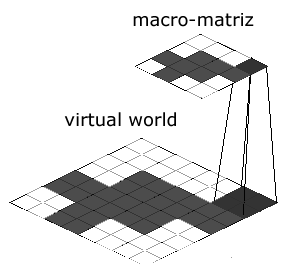
\includegraphics{images/english/mapeamento_macro.png}}
\caption{Mapping the MM to the virtual world: each MM vertex represents several vertices in the virtual world.}
\label{fig:mapeamento_macro}
\end{figure}

The smaller is the MM size, the more vertices in the virtual world will be represented by the same entry in the MM. If the virtual world had {\tt 1000x1000} as its size and the MM had {\tt 10x10} as its size, for instance, it means that each entry of the MM represents 100 vertices in the virtual world. If one of these entries is described in the MM as coast, then there is an area of {\tt 100x100} vertices in the virtual world that must be a coast. When any of those vertices in that particular area of the virtual world is analyzed by the CG, it will work on it and return it with different values, which will result in a coastline for that area, not an area entirely filled with land or water.


\subsubsection{Rendering engine}

The rendering engine draws the created heightmap in the screen. The result is rendered as a triangles mesh that is texturized according to the height value of each vertex in the mesh.


%%%%%%%%%%%%%%%%%%%%%%%%%%%%%%%%%%%%%%%%%%%%%%%%%%%%%%%%%%%%%%%%%%%
\section{Implementation}
\label{sec:implementation}
%%%%%%%%%%%%%%%%%%%%%%%%%%%%%%%%%%%%%%%%%%%%%%%%%%%%%%%%%%%%%%%%%%%

The main problem concerning Charack's implementation was the content generation performed on demand. Based on the fact the user can only see what is inside the visible area, all the content generation algorithms need to take into account {\it only} the information that is available in the user's view. Even though this approach is efficient for resources management (process only the visible elements), it increases the complexity of the content generation algorithms.

The algorithm that generates mountains, for instance, has no way to determine where the mountain ends, because the world outside the user's view technically does not exist yet, it will be generated as the user moves. One approach to solve that problem would be the use of a function that describes the mountain backbone, but this function should not rely on begin/end points, because they could not exist in a certain time. If that function does not need any begin/end points, at least it would have to rely on the position of the user in the virtual world. If the function must be aware of some special points, those points have to be previously processed, which would break the on demand content generation concept.

In addition the algorithms are drastically affected by the fact that the information they receive in a certain time may disappear altogether in the next iteration, since the user can move and change the visible content. Using the example of the mountain generation, a mountain could present an abrupt end, because the points being used for the content generation left the user's view. 

To circumvent these problems the content generation was divided into three main stages: infinite terrain, continents and height generation. The on demand content generation affects differently each of these stages and the problems and solutions related to each stage are described in the following sections. 

%%%%%%%%%%%%%%%%%%%%%%%%%%%%%%%%%%%%%%%%%%%%%%%%%%%%%%%%%%%%%%%%%%%%%
\subsection{Infinite terrain}
%%%%%%%%%%%%%%%%%%%%%%%%%%%%%%%%%%%%%%%%%%%%%%%%%%%%%%%%%%%%%%%%%%%%%

The main idea for the content generation is allow the user to walk in an infinite way, looking at new content each time a significant movement is performed. As the user walks, the tool must be able to identify where the observer is located in the world in order to generate the content around that position. To solve this problem, the player is able to look at the screen and see a slice of the virtual world, but with no explicit divisions, such as cells.
%~\cite{infinicity}.

In order to texturize the sliced data a set of images is interpolated and managed by the shading language GLSL ~\cite{glsl}. The height value of the vertex defines the interpolation weight of each texture. As a consequence, a sand texture has higher weight for vertices featuring a low height value, for instance. Figure ~\ref{fig:set_texturas} shows all the available textures.

\begin{figure}
\centering
\resizebox{8cm}{!}{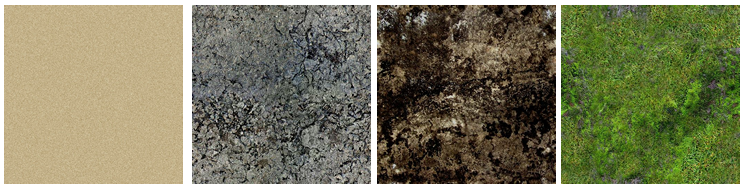
\includegraphics{images/set_texturas.png}}
\caption{Set of image used for terrain texturization}
\label{fig:set_texturas}
\end{figure}


%%%%%%%%%%%%%%%%%%%%%%%%%%%%%%%%%%%%%%%%%%%%%%%%%%%%%%%%%%%%%%%%%%%%%
\subsection{Height generation}
\label{sub:relevo}
%%%%%%%%%%%%%%%%%%%%%%%%%%%%%%%%%%%%%%%%%%%%%%%%%%%%%%%%%%%%%%%%%%%%%

The main idea for the terrain height generation is the use of a parametric function that informs the height value of each vertex. The function is seeded with the point location in the world. As a consequence, the function is able to describe all the height information in the world with no limitation concerning the world size. The processing time is related to the size of the user's view because the function uses the point information to calculate its height value. The height values are generated with a Perlin noise function.


%%%%%%%%%%%%%%%%%%%%%%%%%%%%%%%%%%%%%%%%%%%%%%%%%%%%%%%%%%%%%%%%%%%%%
\subsection{Continents}
%%%%%%%%%%%%%%%%%%%%%%%%%%%%%%%%%%%%%%%%%%%%%%%%%%%%%%%%%%%%%%%%%%%%%

The generation of continents and oceans has been proposed in order to break the monotony of a landscape composed only by land and to increase the similarity of the virtual world with real world landscapes. The solution for the continents generation consists in pre-process the land areas and store that information for later calculations. With that approach, the on demand content generation has been partially broken, since the continents are generated before all the other content, but it ensures a better control over water/land areas. 

The continents generation is based on the planet map creator described in section ~\ref{sec:related-work}. That planet generator was used because it has several parameterization options, such as the possibility to use a seed to manage all the random calculations. Figure ~\ref{fig:torben} {\it (a)}, {\it (b)} and {\it (c)} illustrates the results obtained with the planet generator.

\begin{figure}
\centering
\resizebox{8.2cm}{!}{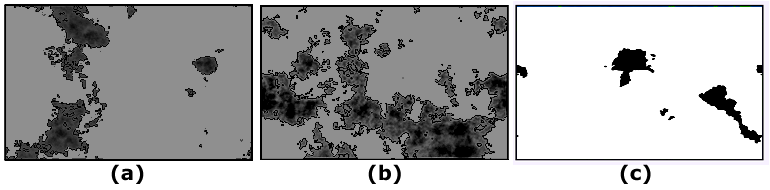
\includegraphics{images/torben_gray.png}}
\caption{Random planets generated with different seeds. (a) and (b) maps featuring height value information; (c) map featuring only information about what is water/land.}
\label{fig:torben}
\end{figure}
%~\cite{torben}


\subsubsection{Problems with continent generation}
\label{sec:visaomicromacro}

As previously explained in section ~\ref{sec:basic-structure}, each entry of the MM is mapped to several vertices in the virtual world. A direct consequence of that mapping process is the generation of large areas featuring straight land lines, as illustrated by figure \ref{fig:ilustracao_mapeamento_macro}. If there were no hardware limitation and if it were possible to generate a MM featuring the exact size of the virtual world, the matrix would contain the necessary resolution for the tool to accurately determine whether a vertex is land or not land, in a ratio of 1:1 (one MM entry is mapped to one world vertex). This approach, however, is not suitable because a matrix with such proportions consumes many resources and processing time. Although the tool allows customization of the MM size, tests showed that a MM featuring {\tt 800x800} as its size has enough information to be processed by all the other algorithms.

\begin{figure}
\centering
\resizebox{8cm}{!}{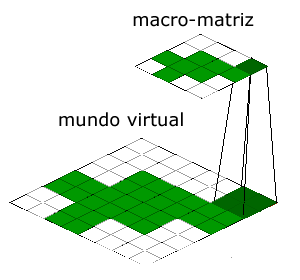
\includegraphics{images/ilustracao_mapeamento_macro.png}}
\caption{The result of no algorithm to generate extra content to fill the discrepancies in the MM mapping process}
\label{fig:ilustracao_mapeamento_macro}
\end{figure}

All images showing Charack results were generated from a world with {\tt 3x3} million vertices and a MM with size of {\tt 800x800}. It means that each MM entry represents 3750 vertices in the virtual world. Figure \ref{fig:ilustracao_mapeamento_macro} illustrates the results obtained by the tool when no algorithm is used to generate extra content to fill the empty spaces in the virtual world. This figure illustrates a place in the virtual world that represents the transition between two different points of the MM (a land point and a water point). To explain what is happening, assume the tool is drawing the world at position {\tt (x, y, z)}, which is the mapping result of an entry {\tt (i, j)} in the MM, which is described as land; as the tool increases the coordinate in order to draw the landscape, each new position is mapped to the MM. If the result of the mapping process of the new coordinate, {\tt (x + 1, y, z))} for instance, is still the entry {\tt (i, j)} in the MM, then the tool will again draw a land vertex on the screen. Assuming that only at point {\tt (x + 10, y, z)} the vertices start being mapped to a different entry in the MM, such as {\tt (i + 1, j)} (assuming it is described as land), then all points before the position {\tt (x + 10, y, z)} are drawn as water and all vertices after that location are drawn as land.

Figure \ref{fig:ilustracao_mapeamento_macro} shows clearly when the world coordinates start being mapped to a different entry in the MM, which is when the tool replaces the land rendering with the water rendering. As a consequence of no algorithm being applied to generate content for that transition area, the user will move along the coastline and will see only straight lines.

\subsubsection{Coastline disturbance}
\label{sec:coastline-disturbance}

The mapping process of the vertices of the virtual world to the MM produces very unrealistic landscapes. A real world beach has a natural curvature and is not likely to have a length of 20 Km in a perfectly straight configuration. Although the objective of this work is not to create photo-realistic landscapes, such unreal beaches are not acceptable. To circumvent this problem, a coastline disturbance is applied to the locations where the mapping process is made between two MM points, one of them described as land and the other one described as water. The algorithm is described below.

The MM has a complete description of what is land and what is water in the virtual world. Each of its entries has a descriptor, which tells the other algorithms what type of terrain one vertex of the virtual world is after it is mapped to the MM. Charack features three types of terrain: water, land (continent) and offshore (land in contact with water). After the continents are pre-processed and stored in the MM, it only contains information about land (continents) and water.

From that moment, the first step of the coastline disturbance algorithm is performed. Using the current MM as its input, the algorithm scan each MM's entries updating the descriptor of all entries that represents coasts. A entry is classified as coast when at least one of its neighbors is water. After the algorithm ends, the MM contains the three types of terrain described before (water, land and offshore). The next step to apply disturbance to the coastline is the content generation based on the descriptor of each MM entry. When the tool is creating content to be drawn on the screen, each vertex being drawn is tested against its descriptor in the MM. If the vertex is mapped to a land entry in the MM, then the function will set a height value for that point. If the vertex is mapped to a water entry in the MM, then the function will set the sea level height to that point. Finally if the vertex is mapped to a offshore entry in the MM, then the function will disturb the land/water information of that vertex, which will result on a non-straight coastline. Figure ~\ref{fig:funcionamento_quebra_linearidade} illustrates the algorithm. 

\begin{figure}
\centering
\resizebox{7.2cm}{!}{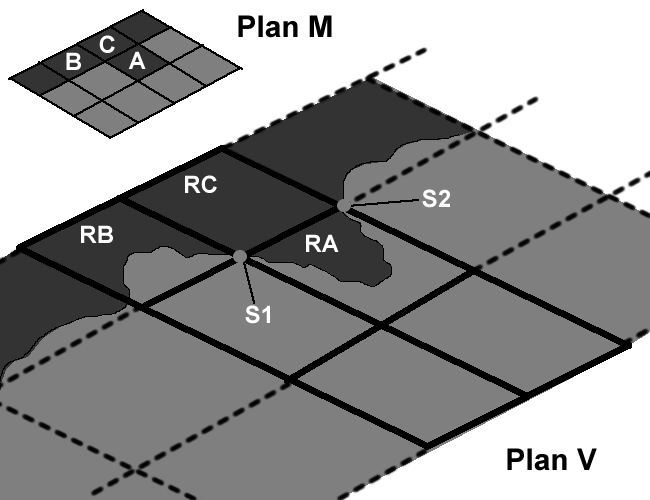
\includegraphics{images/english/funcionamento_quebra_linearidade.png}}
\caption{Coastline disturbance algorithm}
\label{fig:funcionamento_quebra_linearidade}
\end{figure}

The MM entries {\tt A} and {\tt B} have a descriptor indicating that they are classified as a coast. Plan {\tt M} describes the MM and plan {\tt V} describes the result of the mapping process between them. It is not described in the figure, but each block of plan {\tt V} is composed of several vertices, while each block of plan {\tt M} represents only one MM entry. The MM entry {\tt C} is mapped to a massive block of land in the plan {\tt V}, as its descriptor tells the tool that it is a entry described as land. The entry {\tt A} would also be mapped to a massive block of land, but with the intervention of the coastline disturbance algorithm it is mapped to a different configuration. During the content generation for the vertices that are inside the block {\tt RA}, the coastline disturbance algorithm alters the land/water information for each vertex, so that the block will not be composed of land or water vertices only, but a combination of them instead.

The implementation of that process is based on a noise function and random numbers with a parametric function deciding what is land and what is water for all vertices described as a coast in the MM. Using the vertex position in the block {\tt RA}, the function maps that information into a spectrum of values created by a Perlin noise function. What the parametric function does is check if the hash of the vertex being analyzed is inside or outside of the spectrum. The process can be illustrated as a height test of a value against a small heightmap (which is created as a result of the noise spectrum): if the return of the noise function for that vertex is greater than a certain value (which is the granularity of the block being analyzed), then it is classified as land, otherwise it is classified as water. The higher is the granularity of the block, the greater is the amount of land on that location. Figure ~\ref{fig:plot_ruido_quebra_linearidade} illustrates the small heightmap generated by the coastline disturbance algorithm when block {\tt RA} is being processed. 

\begin{figure}
\centering
\resizebox{5cm}{!}{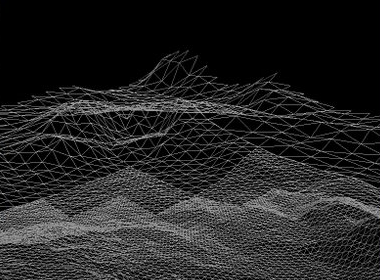
\includegraphics{images/plot_ruido_quebra_linearidade.png}}
\caption{Small heightmap generated by the coastline disturbance algorithm}
\label{fig:plot_ruido_quebra_linearidade}
\end{figure}


\subsubsection{Beaches}

The coastline disturbance algorithm minimizes the problem of unrealistic coastlines, but the outcome is not quite good enough. When Charack is rendering a slice of the world, for each vertex described as land a height value is set it; the same applies to the vertices that are described as water, but in that case the height value is always the same (the sea level). As a direct result of that approach if the tool is rendering a set of vertices which belongs to a mountain and the next vertices are described as water at the MM, the landscape will features a "step". It happens because the mountain backbone was generated very close to the water, which means that its rendering is abruptly interrupted when Charack finds vertices described as water. Although there are cliffs in the real world, they are not present in all coasts. To solve this problem, a special algorithm is applied in order to create beaches in certain locations of the world, which makes the generated landscape looks more realistic.

The beach generation algorithm is performed right before the content is rendered on the screen. After Charack maps the vertices to the MM and after the coastline disturbance algorithm is performed, the result is a heightmap ready to be rendered. The heightmap is treated by the beach creator algorithm before being drawn on the screen, as figure ~\ref{fig:funcionamento_algoritmo_praia}. The procedure scans all the vertices in the map and for each one its distance to a near water vertex is checked. The vertices around the target are mapped directly to the MM, so the only information that is used from the heightmap is the vertex location in the world (which is necessary to map it to the MM). The checking process is performed in four directions (right, left, up and down) and it ends when a water vertex is found or when {\tt N} vertices were analyzed. After that, the four distances are added and used to calculate the height of the beach. The possible results are:

\begin{itemize}
	\item If the vertex has {\tt 4N} as its distance (Figure ~\ref{fig:funcionamento_algoritmo_praia}, point {\tt B}), it means the tool has iterated through the four possible directions and found no water. In this case, the height value for the vertex remains the same. It happens to all the vertices that are within the continent or on the coast but away from the water: they do not belong to the beach area and their height value is defined by the height generator; 
 
	\item If the vertex has a value smaller than {\tt 4N} as its distance (Figure ~\ref{fig:funcionamento_algoritmo_praia}, point {\tt A}), then its height value will be recalculated, because the vertex is located at the beach. The greater is the distance from that vertex to the water vertex, the greater is the height value that will be applied. The height variation is calculated within a range of {\tt [T,B]}, where {\tt T} is the maximum height and {\tt B} is a minimum height value of all vertices in the beach. The result of that approach is a beach featuring higher height values near the continent and lower height values near the water.
\end{itemize}
 
 \begin{figure}
\centering
\resizebox{8.1cm}{!}{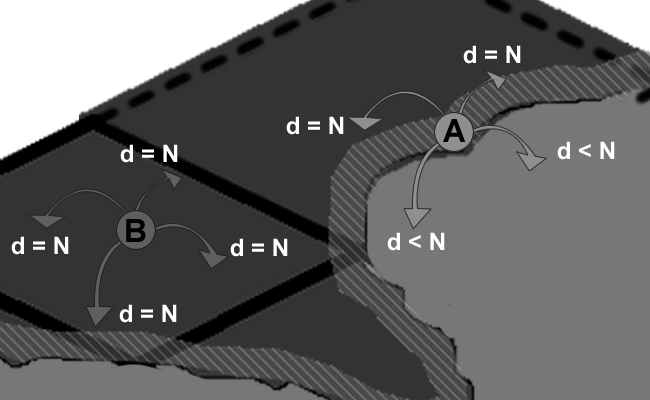
\includegraphics{images/english/funcionamento_algoritmo_praia.png}}
\caption{Beach generation algorithm}
\label{fig:funcionamento_algoritmo_praia}
\end{figure}
 

\begin{figure}
\centering
\resizebox{8cm}{!}{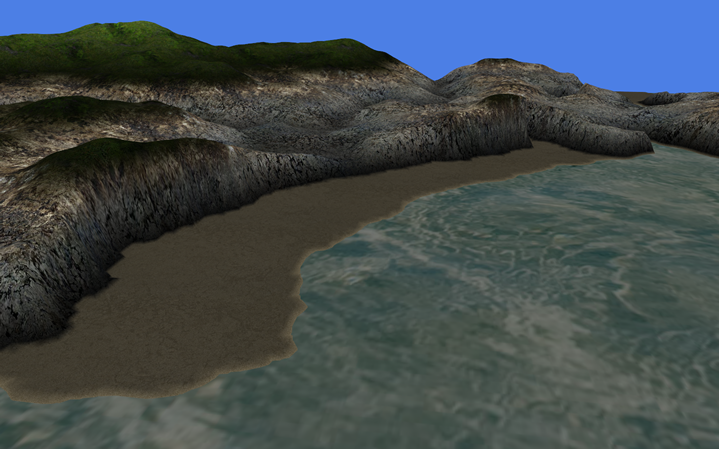
\includegraphics{images/exemplo_praia_complexa.png}}
\caption{Results of the beach generator algorithm}
\label{fig:exemplo_praia_simples}
\end{figure}

Figure ~\ref{fig:exemplo_praia_simples} shows the results of the beach generator algorithm.

\subsubsection{Island generator and beach disturber}

The coastline disturbance and the beach generation algorithms make Charack able to generate more realistic landscapes. The final result, however, presents a well defined pattern, which is unusual to happen in the real world, where the lines and landscapes are more likely to follow a random patterns. If the player walks in the virtual world only through the coast, he would see beaches with the same configuration and no islands along the path. To avoid that problem, two new algorithms are applied to the coastline vertices: beach disturber and island generator.

The \textbf{beach disturber} disturbs the distance used to calculate the water vertices neighboring a certain vertex. Instead of using {\tt N} as value to calculate the distance from the vertex to the water, the beach disturber uses the vertex position as a seed and generates a new value that will be used as the distance. Using this technique, the beach disturber is able to change the size and shape of the beaches, so that certain regions may have a greater amount of sand than others. Figure ~\ref{fig:exemplo_praia_complexa} shows the beach disturber results.

\begin{figure}
\centering
\resizebox{8cm}{!}{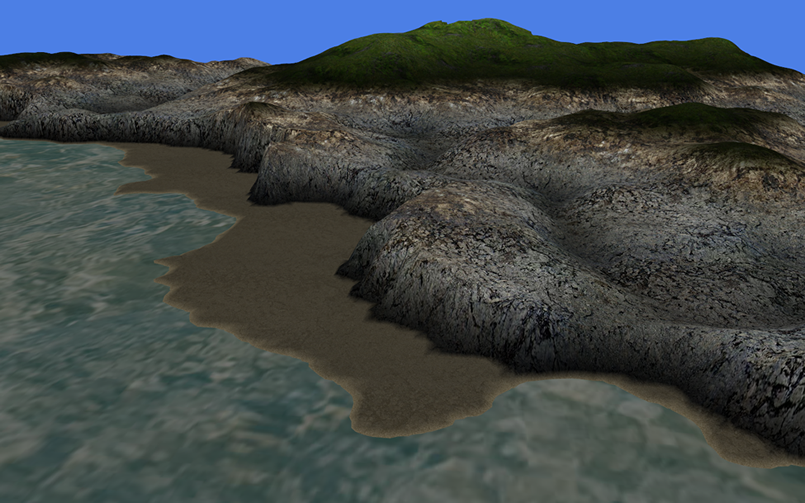
\includegraphics{images/screen_mundo.png}}
\caption{Results of the beach disturber algorithm}
\label{fig:exemplo_praia_complexa}
\end{figure}

The \textbf{island generator} creates land portions in some MM entries. After the MM is created and all the descriptors are configured, the generator iterates through all entries described as coast and for some of them it sets a flag describing that region as a place that features islands. Each vertex mapped to that special regions of the MM has its position used as a hash that is tested against a spectrum created by a noise function. According to the test result, the vertex is classified as land, so a group of vertices classified as land will produce an island. The noise spectrum used for that are different from that one used in the coastline disturbance algorithm, since the expected outcome are small portions of land (islands). Figure ~\ref{fig:exemplo_ilha} shows the island generator results. 

\begin{figure}
\centering
\resizebox{8cm}{!}{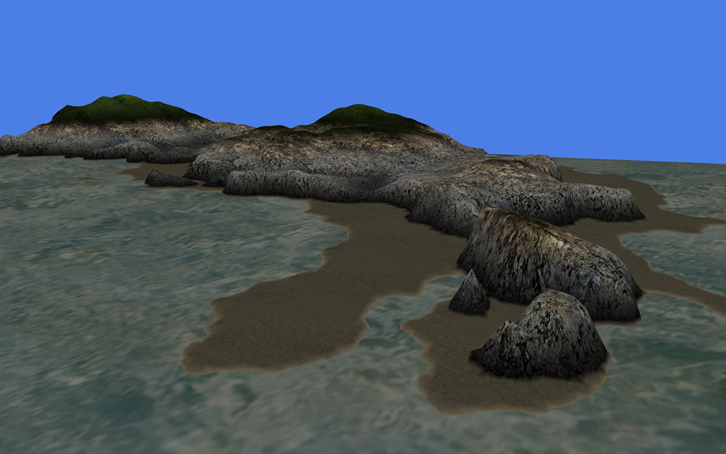
\includegraphics{images/exemplo_ilha.png}}
\caption{Island generated by the island generator (beach area has been influenced by the beach disturber)}
\label{fig:exemplo_ilha}
\end{figure}



%%%%%%%%%%%%%%%%%%%%%%%%%%%%%%%%%%%%%%%%%%%%%%%%%%%%%%%%%%%%%%%%%%%
\section{Results}
\label{sec:results}
%%%%%%%%%%%%%%%%%%%%%%%%%%%%%%%%%%%%%%%%%%%%%%%%%%%%%%%%%%%%%%%%%%%

This section aims to evaluate each of the techniques used in the content generation process, explaining the obtained results for each approach. It is important to highlight that Charack's purpose is not the generation of real or photo-realistic content, but elements that can be used to create a 3D game scene. A result is classified as graphically acceptable if it can be integrated into a game and not surprise the player in a negative way, such as a pyramidal mountain instead of a smooth mountain.

\subsection{Continents evaluation}

The time spent for the continent generation is directly proportional to the size of the specified MM. The reduction of the MM size to {\tt 800x800} yielded significant performance improvements. As a consequence, the smaller is the MM size, the more linear and square are the coastlines of each continent. To avoid that problem, it is possible to adjust the coastline disturbance algorithm in order to make it produce more aggressive changes in the coastlines. Figure ~\ref{fig:charack_final_continentes} shows the continents and oceans generated by the Charack.

\begin{figure}
\centering
\resizebox{8cm}{!}{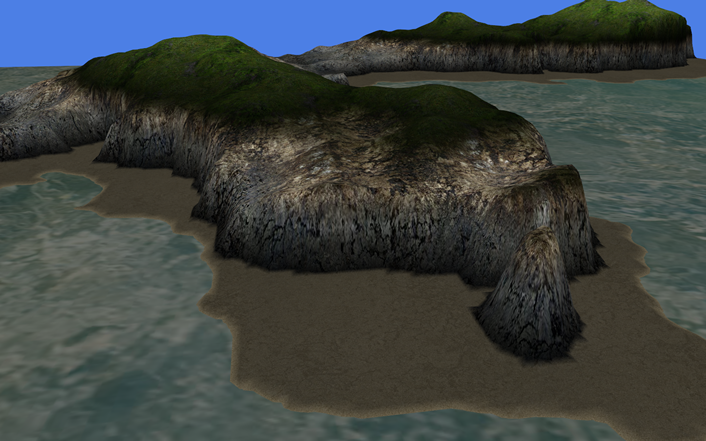
\includegraphics{images/charack_final_continentes.png}}
\caption{Continents and oceans generated by Charack}
\label{fig:charack_final_continentes}
\end{figure}


\subsection{Terrain height evaluation}

The terrain height generated by Charack is fully customizable. The tool has a built-in terrain height generator based on Perlin noise, however it was designed for testing purposes only. The main focus of the present work are the continents and the coastline generation, so any activity related to terrain height generation was very superficial and presents no contribution. Figure ~\ref{fig:charack_final_relevo} shows the terrain height created by the built-in generator.

\begin{figure}
\centering
\resizebox{8cm}{!}{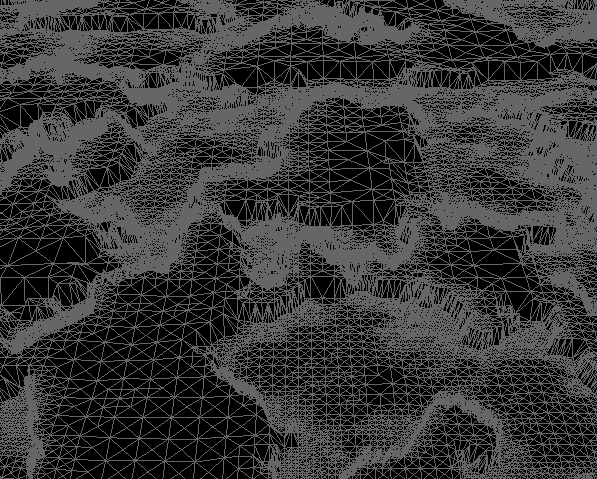
\includegraphics{images/charack_final_relevo.png}}
\caption{Terrain heightmap created by Charack's built-in generator}
\label{fig:charack_final_relevo}
\end{figure}

\subsection{Coastline evaluation}

The coastline generation is composed of two main elements, a global and a local one. The global one only uses data available in the MM in order to create the coastlines, as described in section ~ \ref{sec:visaomicromacro}. The final result for that approach is a unreal straight coastline. Figure ~\ref{fig:charack_final_costa_reta} shows two completely straight coastlines which has no content generation algorithm applied to them. 

\begin{figure}
\centering
\resizebox{8cm}{!}{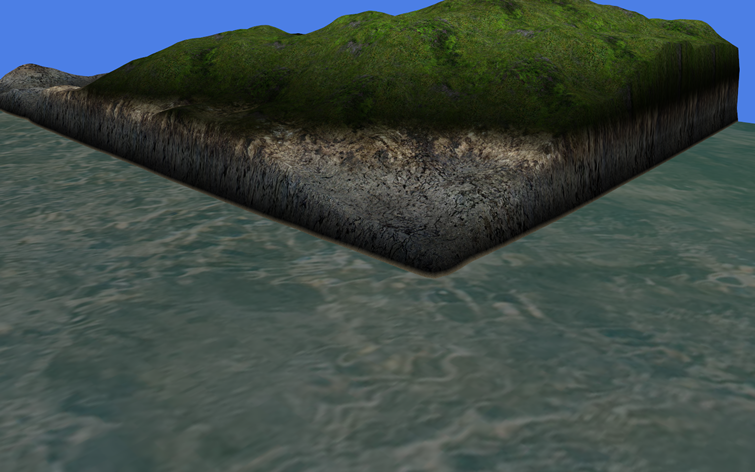
\includegraphics{images/charack_final_costa_reta.png}}
\caption{The interception of two coastlines with no extra content being applied to them}
\label{fig:charack_final_costa_reta}
\end{figure}

After the coastline disturbance algorithm was introduced, Charack started producing more acceptable landscapes. Figures ~\ref{fig:charack_final_costa_1} and ~\ref{fig:charack_final_costa_5} show small bays in some places of the coast. It happened because at those locations the coastline disturbance algorithm created pieces of land towards the ocean and at the same time the beach disturber reduced the amount of sand on the newly created land pieces. Charack is also able to create gulfs, which are large bays, but it is not possible to predict the exact location where those bays will happen because it depends on a set of specific values (location, beach size, etc).

\begin{figure}
\centering
\resizebox{8cm}{!}{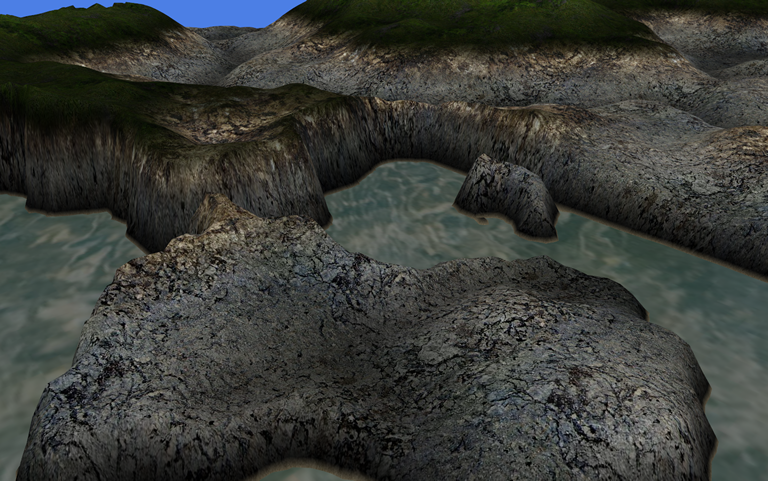
\includegraphics{images/charack_final_costa_1.png}}
\caption{Small bay featuring rocks}
\label{fig:charack_final_costa_1}
\end{figure}

Figures ~\ref{fig:charack_final_costa_3} and ~\ref{fig:charack_final_costa_4} show the final result obtained with the combination of all the previously described algorithms: coastline disturbance, beach disturber and island generator.

%\begin{figure}
%\centering
%\resizebox{8cm}{!}{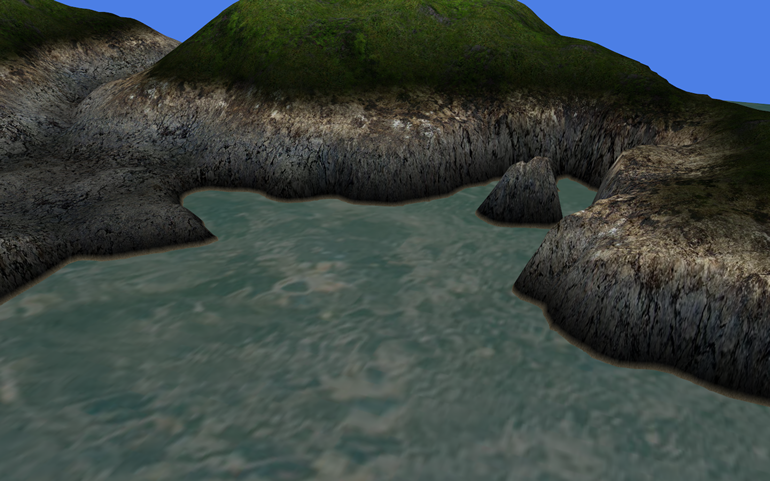
\includegraphics{images/charack_final_costa_2.png}}
%\caption{Small bay featuring no beach area}
%\label{fig:charack_final_costa_2}
%\end{figure}

\begin{figure}
\centering
\resizebox{8cm}{!}{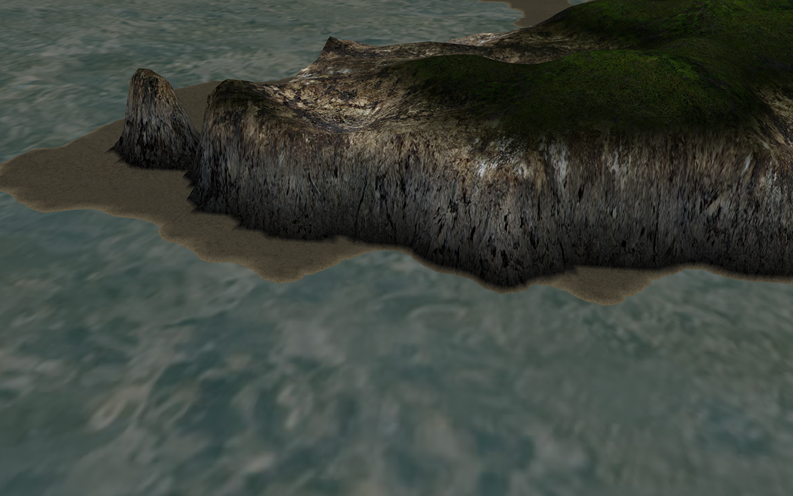
\includegraphics{images/charack_final_costa_3.png}}
\caption{Coastline featuring almost no beach area}
\label{fig:charack_final_costa_3}
\end{figure}

\begin{figure}
\centering
\resizebox{8cm}{!}{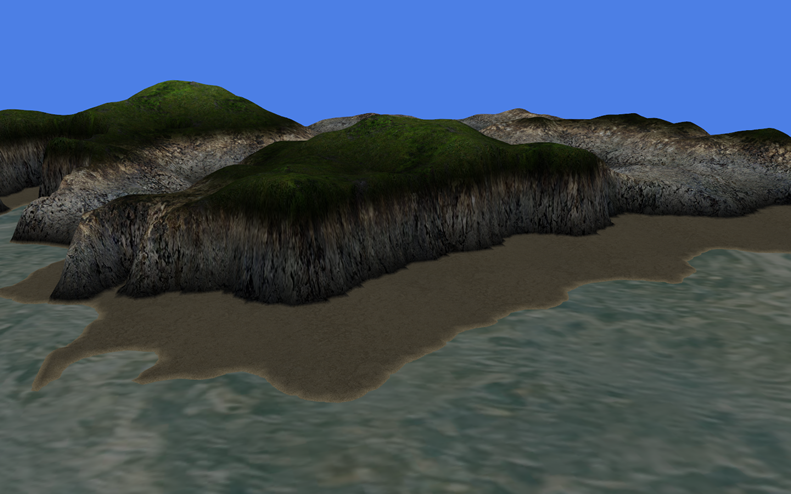
\includegraphics{images/charack_final_costa_4.png}}
\caption{Coastline featuring beaches with different sizes}
\label{fig:charack_final_costa_4}
\end{figure}

\begin{figure}
\centering
\resizebox{8cm}{!}{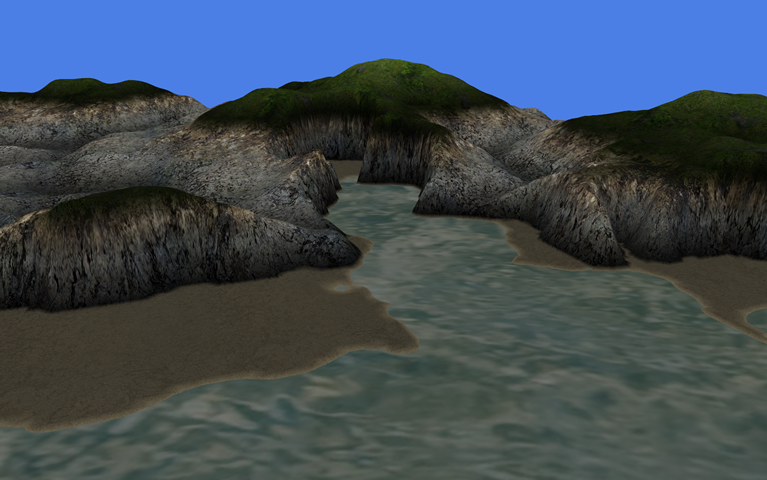
\includegraphics{images/charack_final_costa_5.png}}
\caption{Result of the coastline disturbance algorithm}
\label{fig:charack_final_costa_5}
\end{figure}


%%%%%%%%%%%%%%%%%%%%%%%%%%%%%%%%%%%%%%%%%%%%%%%%%%%%%%%%%%%%%%%%%%%
\section{Conclusion and future work}
\label{sec:conclusion}
%%%%%%%%%%%%%%%%%%%%%%%%%%%%%%%%%%%%%%%%%%%%%%%%%%%%%%%%%%%%%%%%%%%

The automated creation of virtual worlds is one of the available methods that can help developers to create games featuring detailed environments in less time and using fewer resources. Unlike the purely non-automated approaches where a game designer has to design the entirely world, an automated approach is able to generate a complete world with almost none human interference. There are several researches on that subject using different approaches and focusing on a wide range of results.

This paper presented a tool able to generate pseudo-virtual worlds featuring different continents, coastlines and landscapes. Using a combination of algorithms and methods for content management, the tool is able to create beaches, islands, bays and coastlines similar to the ones found in the real world.

One of the Charack's contributions is the ability to generate giant pieces of land focusing on the coastline generation. The development of the present work aimed to handle separately the content generation for all elements in the world (continents, terrains, etc.). The main point in the work is the coastline generation, not the content inside the continents. The final virtual world can be huge: a player with a 100 vertices per second speed in a virtual world generated with the maximum value allowed by a integer will take about 1 year and 3 months to across the whole world.

One suggestion of future work is the enhancement of the height generator, which currently produces a very simple result. Another suggestion is the addition of new types to the MM's descriptors, such as deserts, forests and cities. All the new content can be created tweaking Charack's content generator algorithm in order to produce variations in the current results, such as lowering the height values of all vertices in an area described as a desert, or increasing them in a volcanic area. Another suggestion is to port all the content generation algorithms to the CUBA platform ~\cite{CUDA}. The generation of each world vertex can be calculated separately, so the CUBA parallelism capabilities can be fully used. It will drastically improve Charack's performance and it will allow the generation of a bigger world slice to be displayed in the screen. Another suggestion is the addition of rivers, which can be done with a new MM descriptor and some changes in the content generation algorithm.

%%%%%%%%%%%%%%%%%%%%%%%%%%%%%%%%%%%%%%%%%%%%%%%%%%%%%%%%%%%%%%%%%%%
%\section*{Acknowledgements}
%%%%%%%%%%%%%%%%%%%%%%%%%%%%%%%%%%%%%%%%%%%%%%%%%%%%%%%%%%%%%%%%%%%

%To Cesar, Marilia and my family for all the support.

\bibliographystyle{sbgames}
\bibliography{paper}
\end{document}
